\documentclass[twoside]{book}

% Packages required by doxygen
\usepackage{fixltx2e}
\usepackage{calc}
\usepackage{doxygen}
\usepackage[export]{adjustbox} % also loads graphicx
\usepackage{graphicx}
\usepackage[utf8]{inputenc}
\usepackage{makeidx}
\usepackage{multicol}
\usepackage{multirow}
\PassOptionsToPackage{warn}{textcomp}
\usepackage{textcomp}
\usepackage[nointegrals]{wasysym}
\usepackage[table]{xcolor}

% Font selection
\usepackage[T1]{fontenc}
\usepackage[scaled=.90]{helvet}
\usepackage{courier}
\usepackage{amssymb}
\usepackage{sectsty}
\renewcommand{\familydefault}{\sfdefault}
\allsectionsfont{%
  \fontseries{bc}\selectfont%
  \color{darkgray}%
}
\renewcommand{\DoxyLabelFont}{%
  \fontseries{bc}\selectfont%
  \color{darkgray}%
}
\newcommand{\+}{\discretionary{\mbox{\scriptsize$\hookleftarrow$}}{}{}}

% Page & text layout
\usepackage{geometry}
\geometry{%
  a4paper,%
  top=2.5cm,%
  bottom=2.5cm,%
  left=2.5cm,%
  right=2.5cm%
}
\tolerance=750
\hfuzz=15pt
\hbadness=750
\setlength{\emergencystretch}{15pt}
\setlength{\parindent}{0cm}
\setlength{\parskip}{0.2cm}
\makeatletter
\renewcommand{\paragraph}{%
  \@startsection{paragraph}{4}{0ex}{-1.0ex}{1.0ex}{%
    \normalfont\normalsize\bfseries\SS@parafont%
  }%
}
\renewcommand{\subparagraph}{%
  \@startsection{subparagraph}{5}{0ex}{-1.0ex}{1.0ex}{%
    \normalfont\normalsize\bfseries\SS@subparafont%
  }%
}
\makeatother

% Headers & footers
\usepackage{fancyhdr}
\pagestyle{fancyplain}
\fancyhead[LE]{\fancyplain{}{\bfseries\thepage}}
\fancyhead[CE]{\fancyplain{}{}}
\fancyhead[RE]{\fancyplain{}{\bfseries\leftmark}}
\fancyhead[LO]{\fancyplain{}{\bfseries\rightmark}}
\fancyhead[CO]{\fancyplain{}{}}
\fancyhead[RO]{\fancyplain{}{\bfseries\thepage}}
\fancyfoot[LE]{\fancyplain{}{}}
\fancyfoot[CE]{\fancyplain{}{}}
\fancyfoot[RE]{\fancyplain{}{\bfseries\scriptsize Generated on Fri Oct 9 2015 11\+:55\+:22 for libposemath by Doxygen }}
\fancyfoot[LO]{\fancyplain{}{\bfseries\scriptsize Generated on Fri Oct 9 2015 11\+:55\+:22 for libposemath by Doxygen }}
\fancyfoot[CO]{\fancyplain{}{}}
\fancyfoot[RO]{\fancyplain{}{}}
\renewcommand{\footrulewidth}{0.4pt}
\renewcommand{\chaptermark}[1]{%
  \markboth{#1}{}%
}
\renewcommand{\sectionmark}[1]{%
  \markright{\thesection\ #1}%
}

% Indices & bibliography
\usepackage{natbib}
\usepackage[titles]{tocloft}
\setcounter{tocdepth}{3}
\setcounter{secnumdepth}{5}
\makeindex

% Hyperlinks (required, but should be loaded last)
\usepackage{ifpdf}
\ifpdf
  \usepackage[pdftex,pagebackref=true]{hyperref}
\else
  \usepackage[ps2pdf,pagebackref=true]{hyperref}
\fi
\hypersetup{%
  colorlinks=true,%
  linkcolor=blue,%
  citecolor=blue,%
  unicode%
}

% Custom commands
\newcommand{\clearemptydoublepage}{%
  \newpage{\pagestyle{empty}\cleardoublepage}%
}


%===== C O N T E N T S =====

\begin{document}

% Titlepage & ToC
\hypersetup{pageanchor=false,
             bookmarks=true,
             bookmarksnumbered=true,
             pdfencoding=unicode
            }
\pagenumbering{roman}
\begin{titlepage}
\vspace*{7cm}
\begin{center}%
{\Large libposemath }\\
\vspace*{1cm}
{\large Generated by Doxygen 1.8.9.1}\\
\vspace*{0.5cm}
{\small Fri Oct 9 2015 11:55:22}\\
\end{center}
\end{titlepage}
\clearemptydoublepage
\tableofcontents
\clearemptydoublepage
\pagenumbering{arabic}
\hypersetup{pageanchor=true}

%--- Begin generated contents ---
\chapter{Class Index}
\section{Class List}
Here are the classes, structs, unions and interfaces with brief descriptions\+:\begin{DoxyCompactList}
\item\contentsline{section}{\hyperlink{structPmCartesian}{Pm\+Cartesian} }{\pageref{structPmCartesian}}{}
\item\contentsline{section}{\hyperlink{structPmCircle}{Pm\+Circle} }{\pageref{structPmCircle}}{}
\item\contentsline{section}{\hyperlink{structPmCylindrical}{Pm\+Cylindrical} }{\pageref{structPmCylindrical}}{}
\item\contentsline{section}{\hyperlink{structPmEulerZyx}{Pm\+Euler\+Zyx} }{\pageref{structPmEulerZyx}}{}
\item\contentsline{section}{\hyperlink{structPmEulerZyz}{Pm\+Euler\+Zyz} }{\pageref{structPmEulerZyz}}{}
\item\contentsline{section}{\hyperlink{structPmHomogeneous}{Pm\+Homogeneous} }{\pageref{structPmHomogeneous}}{}
\item\contentsline{section}{\hyperlink{structPmLine}{Pm\+Line} }{\pageref{structPmLine}}{}
\item\contentsline{section}{\hyperlink{structPmPose}{Pm\+Pose} }{\pageref{structPmPose}}{}
\item\contentsline{section}{\hyperlink{structPmQuaternion}{Pm\+Quaternion} }{\pageref{structPmQuaternion}}{}
\item\contentsline{section}{\hyperlink{structPmRotationMatrix}{Pm\+Rotation\+Matrix} }{\pageref{structPmRotationMatrix}}{}
\item\contentsline{section}{\hyperlink{structPmRotationVector}{Pm\+Rotation\+Vector} }{\pageref{structPmRotationVector}}{}
\item\contentsline{section}{\hyperlink{structPmRpy}{Pm\+Rpy} }{\pageref{structPmRpy}}{}
\item\contentsline{section}{\hyperlink{structPmSpherical}{Pm\+Spherical} }{\pageref{structPmSpherical}}{}
\item\contentsline{section}{\hyperlink{structPmXya}{Pm\+Xya} }{\pageref{structPmXya}}{}
\item\contentsline{section}{\hyperlink{structVECTOR}{V\+E\+C\+T\+O\+R} }{\pageref{structVECTOR}}{}
\end{DoxyCompactList}

\chapter{Class Documentation}
\hypertarget{structPmCartesian}{}\section{Pm\+Cartesian Struct Reference}
\label{structPmCartesian}\index{Pm\+Cartesian@{Pm\+Cartesian}}
\subsection*{Public Attributes}
\begin{DoxyCompactItemize}
\item 
\hypertarget{structPmCartesian_a145c5fdd25037b86b5fa002e7d3e03b2}{}double {\bfseries x}\label{structPmCartesian_a145c5fdd25037b86b5fa002e7d3e03b2}

\item 
\hypertarget{structPmCartesian_a4d6af7d58c93464d7caefde53f35e8b2}{}double {\bfseries y}\label{structPmCartesian_a4d6af7d58c93464d7caefde53f35e8b2}

\item 
\hypertarget{structPmCartesian_a7bcca0d664a97cc106b726b6bf67ed89}{}double {\bfseries z}\label{structPmCartesian_a7bcca0d664a97cc106b726b6bf67ed89}

\end{DoxyCompactItemize}


The documentation for this struct was generated from the following file\+:\begin{DoxyCompactItemize}
\item 
/home/home/dave/src/libposemath-\/2014.\+04.\+29/src/posemath/posemath.\+h\end{DoxyCompactItemize}

\hypertarget{structPmCircle}{}\section{Pm\+Circle Struct Reference}
\label{structPmCircle}\index{Pm\+Circle@{Pm\+Circle}}


Collaboration diagram for Pm\+Circle\+:
\nopagebreak
\begin{figure}[H]
\begin{center}
\leavevmode
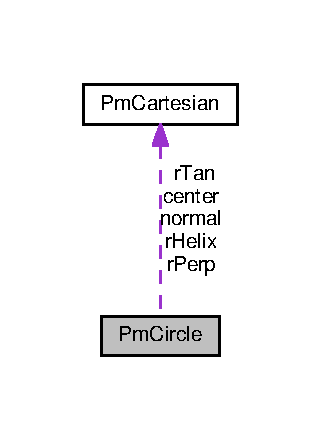
\includegraphics[width=154pt]{structPmCircle__coll__graph}
\end{center}
\end{figure}
\subsection*{Public Attributes}
\begin{DoxyCompactItemize}
\item 
\hypertarget{structPmCircle_abb8e717dcdf600e451cdb8153e37880c}{}\hyperlink{structPmCartesian}{Pm\+Cartesian} {\bfseries center}\label{structPmCircle_abb8e717dcdf600e451cdb8153e37880c}

\item 
\hypertarget{structPmCircle_abe570b56562fc0b35cd9d069b290970c}{}\hyperlink{structPmCartesian}{Pm\+Cartesian} {\bfseries normal}\label{structPmCircle_abe570b56562fc0b35cd9d069b290970c}

\item 
\hypertarget{structPmCircle_af65b788b063c25dae7d256577e1ed1b7}{}\hyperlink{structPmCartesian}{Pm\+Cartesian} {\bfseries r\+Tan}\label{structPmCircle_af65b788b063c25dae7d256577e1ed1b7}

\item 
\hypertarget{structPmCircle_a95a83221908ef57b4e5df2f52aa45636}{}\hyperlink{structPmCartesian}{Pm\+Cartesian} {\bfseries r\+Perp}\label{structPmCircle_a95a83221908ef57b4e5df2f52aa45636}

\item 
\hypertarget{structPmCircle_adbe1a652cb701779442fee961a4b092e}{}\hyperlink{structPmCartesian}{Pm\+Cartesian} {\bfseries r\+Helix}\label{structPmCircle_adbe1a652cb701779442fee961a4b092e}

\item 
\hypertarget{structPmCircle_a79a2ee314d4f0cb0283b69864ca58d88}{}double {\bfseries radius}\label{structPmCircle_a79a2ee314d4f0cb0283b69864ca58d88}

\item 
\hypertarget{structPmCircle_a45857969dbf5f2a349ccbeff556d1385}{}double {\bfseries angle}\label{structPmCircle_a45857969dbf5f2a349ccbeff556d1385}

\item 
\hypertarget{structPmCircle_aea2c69e2bc01682e81dfc1b8a4b5b56e}{}double {\bfseries spiral}\label{structPmCircle_aea2c69e2bc01682e81dfc1b8a4b5b56e}

\end{DoxyCompactItemize}


The documentation for this struct was generated from the following file\+:\begin{DoxyCompactItemize}
\item 
/home/home/dave/src/libposemath-\/2014.\+04.\+29/src/posemath/posemath.\+h\end{DoxyCompactItemize}

\hypertarget{structPmCylindrical}{}\section{Pm\+Cylindrical Struct Reference}
\label{structPmCylindrical}\index{Pm\+Cylindrical@{Pm\+Cylindrical}}
\subsection*{Public Attributes}
\begin{DoxyCompactItemize}
\item 
\hypertarget{structPmCylindrical_af39d13ff1b623c783197358f89b5f3cb}{}double {\bfseries theta}\label{structPmCylindrical_af39d13ff1b623c783197358f89b5f3cb}

\item 
\hypertarget{structPmCylindrical_a5ff182da8d4f7f3e9a5a4de3a8a63005}{}double {\bfseries r}\label{structPmCylindrical_a5ff182da8d4f7f3e9a5a4de3a8a63005}

\item 
\hypertarget{structPmCylindrical_a099a6f4e34a7993b442af4cf33abf41e}{}double {\bfseries z}\label{structPmCylindrical_a099a6f4e34a7993b442af4cf33abf41e}

\end{DoxyCompactItemize}


The documentation for this struct was generated from the following file\+:\begin{DoxyCompactItemize}
\item 
/home/home/dave/src/libposemath-\/2014.\+04.\+29/src/posemath/posemath.\+h\end{DoxyCompactItemize}

\hypertarget{structPmEulerZyx}{}\section{Pm\+Euler\+Zyx Struct Reference}
\label{structPmEulerZyx}\index{Pm\+Euler\+Zyx@{Pm\+Euler\+Zyx}}
\subsection*{Public Attributes}
\begin{DoxyCompactItemize}
\item 
\hypertarget{structPmEulerZyx_ad631af580a7537ca9bb6cf49cf0a678d}{}double {\bfseries z}\label{structPmEulerZyx_ad631af580a7537ca9bb6cf49cf0a678d}

\item 
\hypertarget{structPmEulerZyx_af5fa3ee219a2a0fa530aa052ea419127}{}double {\bfseries y}\label{structPmEulerZyx_af5fa3ee219a2a0fa530aa052ea419127}

\item 
\hypertarget{structPmEulerZyx_a05f63fddcbebd46ff61343ad5741fa35}{}double {\bfseries x}\label{structPmEulerZyx_a05f63fddcbebd46ff61343ad5741fa35}

\end{DoxyCompactItemize}


The documentation for this struct was generated from the following file\+:\begin{DoxyCompactItemize}
\item 
/home/home/dave/src/libposemath-\/2014.\+04.\+29/src/posemath/posemath.\+h\end{DoxyCompactItemize}

\hypertarget{structPmEulerZyz}{}\section{Pm\+Euler\+Zyz Struct Reference}
\label{structPmEulerZyz}\index{Pm\+Euler\+Zyz@{Pm\+Euler\+Zyz}}
\subsection*{Public Attributes}
\begin{DoxyCompactItemize}
\item 
\hypertarget{structPmEulerZyz_aca652d0f1857cc5de5091226e92d558c}{}double {\bfseries z}\label{structPmEulerZyz_aca652d0f1857cc5de5091226e92d558c}

\item 
\hypertarget{structPmEulerZyz_ac60535f04b17bbaffc8314eb277e49a7}{}double {\bfseries y}\label{structPmEulerZyz_ac60535f04b17bbaffc8314eb277e49a7}

\item 
\hypertarget{structPmEulerZyz_abe2ad8e53ce0d8c01129de13b64aa580}{}double {\bfseries zp}\label{structPmEulerZyz_abe2ad8e53ce0d8c01129de13b64aa580}

\end{DoxyCompactItemize}


The documentation for this struct was generated from the following file\+:\begin{DoxyCompactItemize}
\item 
/home/home/dave/src/libposemath-\/2014.\+04.\+29/src/posemath/posemath.\+h\end{DoxyCompactItemize}

\hypertarget{structPmHomogeneous}{}\section{Pm\+Homogeneous Struct Reference}
\label{structPmHomogeneous}\index{Pm\+Homogeneous@{Pm\+Homogeneous}}


Collaboration diagram for Pm\+Homogeneous\+:
\nopagebreak
\begin{figure}[H]
\begin{center}
\leavevmode
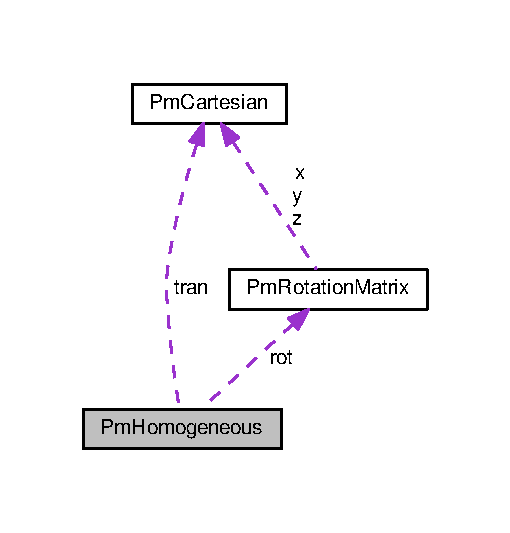
\includegraphics[width=245pt]{structPmHomogeneous__coll__graph}
\end{center}
\end{figure}
\subsection*{Public Attributes}
\begin{DoxyCompactItemize}
\item 
\hypertarget{structPmHomogeneous_ae324a04f02ac177db35cbcb919a64f1e}{}\hyperlink{structPmCartesian}{Pm\+Cartesian} {\bfseries tran}\label{structPmHomogeneous_ae324a04f02ac177db35cbcb919a64f1e}

\item 
\hypertarget{structPmHomogeneous_a697360580aaa1b6a697182fc67349ed2}{}\hyperlink{structPmRotationMatrix}{Pm\+Rotation\+Matrix} {\bfseries rot}\label{structPmHomogeneous_a697360580aaa1b6a697182fc67349ed2}

\end{DoxyCompactItemize}


The documentation for this struct was generated from the following file\+:\begin{DoxyCompactItemize}
\item 
/home/home/dave/src/libposemath-\/2014.\+04.\+29/src/posemath/posemath.\+h\end{DoxyCompactItemize}

\hypertarget{structPmLine}{}\section{Pm\+Line Struct Reference}
\label{structPmLine}\index{Pm\+Line@{Pm\+Line}}


Collaboration diagram for Pm\+Line\+:
\nopagebreak
\begin{figure}[H]
\begin{center}
\leavevmode
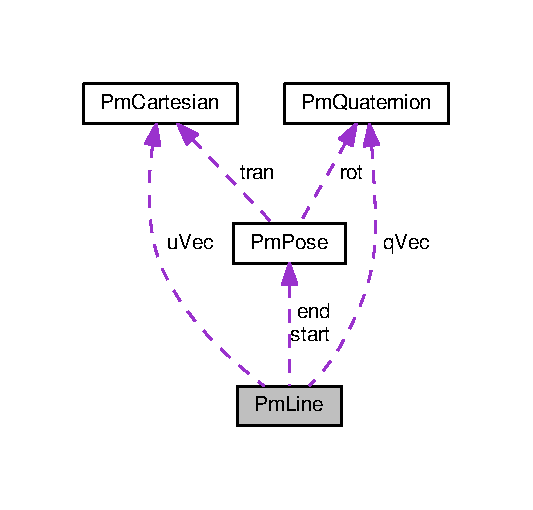
\includegraphics[width=256pt]{structPmLine__coll__graph}
\end{center}
\end{figure}
\subsection*{Public Attributes}
\begin{DoxyCompactItemize}
\item 
\hypertarget{structPmLine_ac0c0df1d38527e3f726b3062a7d625c0}{}\hyperlink{structPmPose}{Pm\+Pose} {\bfseries start}\label{structPmLine_ac0c0df1d38527e3f726b3062a7d625c0}

\item 
\hypertarget{structPmLine_a9a78b09ef9d8f9e631a06663eb2aa7cd}{}\hyperlink{structPmPose}{Pm\+Pose} {\bfseries end}\label{structPmLine_a9a78b09ef9d8f9e631a06663eb2aa7cd}

\item 
\hypertarget{structPmLine_a9bc27c01a819b140c5aad8db84aa8c23}{}\hyperlink{structPmCartesian}{Pm\+Cartesian} {\bfseries u\+Vec}\label{structPmLine_a9bc27c01a819b140c5aad8db84aa8c23}

\item 
\hypertarget{structPmLine_a1b59db8f7621b457b22ec19388c9be38}{}\hyperlink{structPmQuaternion}{Pm\+Quaternion} {\bfseries q\+Vec}\label{structPmLine_a1b59db8f7621b457b22ec19388c9be38}

\item 
\hypertarget{structPmLine_aef03bfafda7c6a4d2870c3ee4f8f7109}{}double {\bfseries tmag}\label{structPmLine_aef03bfafda7c6a4d2870c3ee4f8f7109}

\item 
\hypertarget{structPmLine_a4b42d77106059d3617b5be0c1f04ae84}{}double {\bfseries rmag}\label{structPmLine_a4b42d77106059d3617b5be0c1f04ae84}

\item 
\hypertarget{structPmLine_a26bd5b75d2e65d5d816fecca7257ba86}{}int {\bfseries tmag\+\_\+is\+\_\+greater\+\_\+than\+\_\+rmag}\label{structPmLine_a26bd5b75d2e65d5d816fecca7257ba86}

\item 
\hypertarget{structPmLine_a8cee13824dcdc4eb04b187c2459d58f8}{}int {\bfseries tmag\+\_\+zero}\label{structPmLine_a8cee13824dcdc4eb04b187c2459d58f8}

\item 
\hypertarget{structPmLine_ae1eee01e0e7a04c0bc9546f5f3d4497a}{}int {\bfseries rmag\+\_\+zero}\label{structPmLine_ae1eee01e0e7a04c0bc9546f5f3d4497a}

\end{DoxyCompactItemize}


The documentation for this struct was generated from the following file\+:\begin{DoxyCompactItemize}
\item 
/home/home/dave/src/libposemath-\/2014.\+04.\+29/src/posemath/posemath.\+h\end{DoxyCompactItemize}

\hypertarget{structPmPose}{}\section{Pm\+Pose Struct Reference}
\label{structPmPose}\index{Pm\+Pose@{Pm\+Pose}}


Collaboration diagram for Pm\+Pose\+:
\nopagebreak
\begin{figure}[H]
\begin{center}
\leavevmode
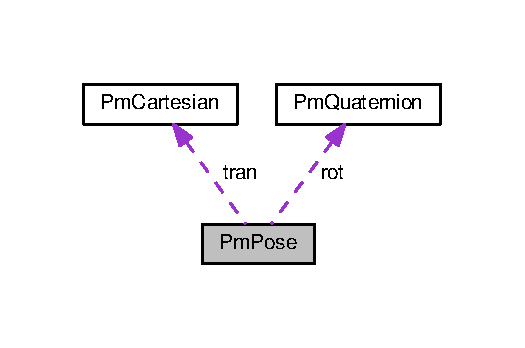
\includegraphics[width=252pt]{structPmPose__coll__graph}
\end{center}
\end{figure}
\subsection*{Public Attributes}
\begin{DoxyCompactItemize}
\item 
\hypertarget{structPmPose_a1e6e45c5385628f5fc385cabe1f5294b}{}\hyperlink{structPmCartesian}{Pm\+Cartesian} {\bfseries tran}\label{structPmPose_a1e6e45c5385628f5fc385cabe1f5294b}

\item 
\hypertarget{structPmPose_acf1225d1b132e7945d4ac2c69711c1fe}{}\hyperlink{structPmQuaternion}{Pm\+Quaternion} {\bfseries rot}\label{structPmPose_acf1225d1b132e7945d4ac2c69711c1fe}

\end{DoxyCompactItemize}


The documentation for this struct was generated from the following file\+:\begin{DoxyCompactItemize}
\item 
/home/home/dave/src/libposemath-\/2014.\+04.\+29/src/posemath/posemath.\+h\end{DoxyCompactItemize}

\hypertarget{structPmQuaternion}{}\section{Pm\+Quaternion Struct Reference}
\label{structPmQuaternion}\index{Pm\+Quaternion@{Pm\+Quaternion}}
\subsection*{Public Attributes}
\begin{DoxyCompactItemize}
\item 
\hypertarget{structPmQuaternion_abff23016cfafd41abab7e0791816f15c}{}double {\bfseries s}\label{structPmQuaternion_abff23016cfafd41abab7e0791816f15c}

\item 
\hypertarget{structPmQuaternion_a84b05f2af41e52cfc051d77c6cc53234}{}double {\bfseries x}\label{structPmQuaternion_a84b05f2af41e52cfc051d77c6cc53234}

\item 
\hypertarget{structPmQuaternion_a6d683884d3ff0ba53f1af36151e465b2}{}double {\bfseries y}\label{structPmQuaternion_a6d683884d3ff0ba53f1af36151e465b2}

\item 
\hypertarget{structPmQuaternion_a5dce4b60d3650e811e50d782320ffaae}{}double {\bfseries z}\label{structPmQuaternion_a5dce4b60d3650e811e50d782320ffaae}

\end{DoxyCompactItemize}


The documentation for this struct was generated from the following file\+:\begin{DoxyCompactItemize}
\item 
/home/home/dave/src/libposemath-\/2014.\+04.\+29/src/posemath/posemath.\+h\end{DoxyCompactItemize}

\hypertarget{structPmRotationMatrix}{}\section{Pm\+Rotation\+Matrix Struct Reference}
\label{structPmRotationMatrix}\index{Pm\+Rotation\+Matrix@{Pm\+Rotation\+Matrix}}


Collaboration diagram for Pm\+Rotation\+Matrix\+:
\nopagebreak
\begin{figure}[H]
\begin{center}
\leavevmode
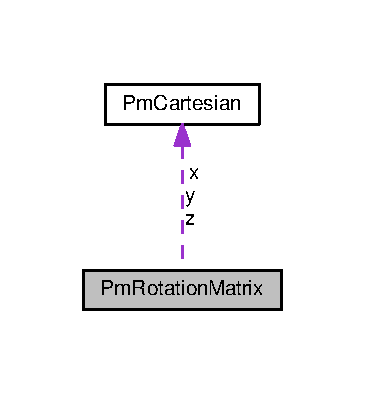
\includegraphics[width=175pt]{structPmRotationMatrix__coll__graph}
\end{center}
\end{figure}
\subsection*{Public Attributes}
\begin{DoxyCompactItemize}
\item 
\hypertarget{structPmRotationMatrix_a2e78c81df93428e13cc0dbf7dcecb16a}{}\hyperlink{structPmCartesian}{Pm\+Cartesian} {\bfseries x}\label{structPmRotationMatrix_a2e78c81df93428e13cc0dbf7dcecb16a}

\item 
\hypertarget{structPmRotationMatrix_a3c31afa8fde83fca9611047239689de3}{}\hyperlink{structPmCartesian}{Pm\+Cartesian} {\bfseries y}\label{structPmRotationMatrix_a3c31afa8fde83fca9611047239689de3}

\item 
\hypertarget{structPmRotationMatrix_a6489b0699ca4582f7f6da5850fe6271d}{}\hyperlink{structPmCartesian}{Pm\+Cartesian} {\bfseries z}\label{structPmRotationMatrix_a6489b0699ca4582f7f6da5850fe6271d}

\end{DoxyCompactItemize}


The documentation for this struct was generated from the following file\+:\begin{DoxyCompactItemize}
\item 
/home/home/dave/src/libposemath-\/2014.\+04.\+29/src/posemath/posemath.\+h\end{DoxyCompactItemize}

\hypertarget{structPmRotationVector}{}\section{Pm\+Rotation\+Vector Struct Reference}
\label{structPmRotationVector}\index{Pm\+Rotation\+Vector@{Pm\+Rotation\+Vector}}
\subsection*{Public Attributes}
\begin{DoxyCompactItemize}
\item 
\hypertarget{structPmRotationVector_ab52f2e4b958a2d38ce18ef7abee2a277}{}double {\bfseries s}\label{structPmRotationVector_ab52f2e4b958a2d38ce18ef7abee2a277}

\item 
\hypertarget{structPmRotationVector_a5cbee5c6028a38d43252d885b6d63ca8}{}double {\bfseries x}\label{structPmRotationVector_a5cbee5c6028a38d43252d885b6d63ca8}

\item 
\hypertarget{structPmRotationVector_ae19524f26cdd3012a6b5cc1c043c6083}{}double {\bfseries y}\label{structPmRotationVector_ae19524f26cdd3012a6b5cc1c043c6083}

\item 
\hypertarget{structPmRotationVector_a6c5fe9034f23157dd6b42286a015c6fe}{}double {\bfseries z}\label{structPmRotationVector_a6c5fe9034f23157dd6b42286a015c6fe}

\end{DoxyCompactItemize}


The documentation for this struct was generated from the following file\+:\begin{DoxyCompactItemize}
\item 
/home/home/dave/src/libposemath-\/2014.\+04.\+29/src/posemath/posemath.\+h\end{DoxyCompactItemize}

\hypertarget{structPmRpy}{}\section{Pm\+Rpy Struct Reference}
\label{structPmRpy}\index{Pm\+Rpy@{Pm\+Rpy}}
\subsection*{Public Attributes}
\begin{DoxyCompactItemize}
\item 
\hypertarget{structPmRpy_ad7a7492e7d738eeead795f7447e29fcc}{}double {\bfseries r}\label{structPmRpy_ad7a7492e7d738eeead795f7447e29fcc}

\item 
\hypertarget{structPmRpy_a23b81486467f530713155cbd67ffc7c9}{}double {\bfseries p}\label{structPmRpy_a23b81486467f530713155cbd67ffc7c9}

\item 
\hypertarget{structPmRpy_a64dbc66f55c70e322a8488145e21c8c9}{}double {\bfseries y}\label{structPmRpy_a64dbc66f55c70e322a8488145e21c8c9}

\end{DoxyCompactItemize}


The documentation for this struct was generated from the following file\+:\begin{DoxyCompactItemize}
\item 
/home/home/dave/src/libposemath-\/2014.\+04.\+29/src/posemath/posemath.\+h\end{DoxyCompactItemize}

\hypertarget{structPmSpherical}{}\section{Pm\+Spherical Struct Reference}
\label{structPmSpherical}\index{Pm\+Spherical@{Pm\+Spherical}}
\subsection*{Public Attributes}
\begin{DoxyCompactItemize}
\item 
\hypertarget{structPmSpherical_a478a5d41a8dcda4ae679dfb22f6bfd33}{}double {\bfseries theta}\label{structPmSpherical_a478a5d41a8dcda4ae679dfb22f6bfd33}

\item 
\hypertarget{structPmSpherical_a9945a29e9bc074dc95fb7613ed46a541}{}double {\bfseries phi}\label{structPmSpherical_a9945a29e9bc074dc95fb7613ed46a541}

\item 
\hypertarget{structPmSpherical_a7b17ba0456829680b73ec5e2a1bf3833}{}double {\bfseries r}\label{structPmSpherical_a7b17ba0456829680b73ec5e2a1bf3833}

\end{DoxyCompactItemize}


The documentation for this struct was generated from the following file\+:\begin{DoxyCompactItemize}
\item 
/home/home/dave/src/libposemath-\/2014.\+04.\+29/src/posemath/posemath.\+h\end{DoxyCompactItemize}

\hypertarget{structPmXya}{}\section{Pm\+Xya Struct Reference}
\label{structPmXya}\index{Pm\+Xya@{Pm\+Xya}}
\subsection*{Public Attributes}
\begin{DoxyCompactItemize}
\item 
\hypertarget{structPmXya_aa736345bf65d14e763ac4e7b225c59cc}{}double {\bfseries x}\label{structPmXya_aa736345bf65d14e763ac4e7b225c59cc}

\item 
\hypertarget{structPmXya_af9611e4556bc5a1d04192cff3ddb7203}{}double {\bfseries y}\label{structPmXya_af9611e4556bc5a1d04192cff3ddb7203}

\item 
\hypertarget{structPmXya_aa39eb0bed993ac3be680a64c04d58200}{}double {\bfseries a}\label{structPmXya_aa39eb0bed993ac3be680a64c04d58200}

\end{DoxyCompactItemize}


The documentation for this struct was generated from the following file\+:\begin{DoxyCompactItemize}
\item 
/home/home/dave/src/libposemath-\/2014.\+04.\+29/src/posemath/posemath.\+h\end{DoxyCompactItemize}

\hypertarget{structVECTOR}{}\section{V\+E\+C\+T\+O\+R Struct Reference}
\label{structVECTOR}\index{V\+E\+C\+T\+O\+R@{V\+E\+C\+T\+O\+R}}
\subsection*{Public Attributes}
\begin{DoxyCompactItemize}
\item 
\hypertarget{structVECTOR_a3d2ce826d744d2ddeb45f0b8e8b0cf63}{}double {\bfseries x}\label{structVECTOR_a3d2ce826d744d2ddeb45f0b8e8b0cf63}

\item 
\hypertarget{structVECTOR_a8aed039b215526167c1e96132d9a4101}{}double {\bfseries y}\label{structVECTOR_a8aed039b215526167c1e96132d9a4101}

\item 
\hypertarget{structVECTOR_ad848a8f4b993fec31f80e374ec7a154b}{}double {\bfseries z}\label{structVECTOR_ad848a8f4b993fec31f80e374ec7a154b}

\end{DoxyCompactItemize}


The documentation for this struct was generated from the following file\+:\begin{DoxyCompactItemize}
\item 
/home/home/dave/src/libposemath-\/2014.\+04.\+29/src/posemath/testpmcpp.\+cc\end{DoxyCompactItemize}

%--- End generated contents ---

% Index
\backmatter
\newpage
\phantomsection
\clearemptydoublepage
\addcontentsline{toc}{chapter}{Index}
\printindex

\end{document}
